%%%%%%%%%%%%%%%%%%%%%%%%%%%%%%%%%%%%%%%%%
% Jacobs Landscape Poster
% LaTeX Template
% Version 1.1 (14/06/14)
%
% Created by:
% Computational Physics and Biophysics Group, Jacobs University
% https://teamwork.jacobs-university.de:8443/confluence/display/CoPandBiG/LaTeX+Poster
% 
% Further modified by:
% Nathaniel Johnston (nathaniel@njohnston.ca)
%
% This template has been downloaded from:
% http://www.LaTeXTemplates.com
%
% License:
% CC BY-NC-SA 3.0 (http://creativecommons.org/licenses/by-nc-sa/3.0/)
%
%%%%%%%%%%%%%%%%%%%%%%%%%%%%%%%%%%%%%%%%%

%----------------------------------------------------------------------------------------
%	PACKAGES AND OTHER DOCUMENT CONFIGURATIONS
%----------------------------------------------------------------------------------------

\documentclass[final]{beamer}

\usepackage[scale=1.0]{beamerposter} % Use the beamerposter package for laying out the poster
\usepackage[acronym,toc]{glossaries}
\newacronym[longplural={metric tons of heavy metal}]{MTHM}{MTHM}{metric ton of heavy metal}
\newacronym{ABM}{ABM}{agent-based modeling}
\newacronym{ACDIS}{ACDIS}{Program in Arms Control \& Domestic and International Security}
\newacronym{AHTR}{AHTR}{Advanced High Temperature Reactor}
\newacronym{ANDRA}{ANDRA}{Agence Nationale pour la gestion des D\'echets RAdioactifs, the French National Agency for Radioactive Waste Management}
\newacronym{ANL}{ANL}{Argonne National Laboratory}
\newacronym{API}{API}{application programming interface}
\newacronym{ARCH}{ARCH}{autoregressive conditional heteroskedastic}
\newacronym{ARE}{ARE}{Aircraft Reactor Experiment}
\newacronym{ARFC}{ARFC}{Advanced Reactors and Fuel Cycles}
\newacronym{ARMA}{ARMA}{autoregressive moving average}
\newacronym{ASME}{ASME}{American Society of Mechanical Engineers}
\newacronym{ATWS}{ATWS}{Anticipated Transient Without Scram}
\newacronym{BDBE}{BDBE}{Beyond Design Basis Event}
\newacronym{BIDS}{BIDS}{Berkeley Institute for Data Science}
\newacronym{BOL}{BOL}{Beginning-of-Life}
\newacronym{BSD}{BSD}{Berkeley Software Distribution}
\newacronym{CAFCA}{CAFCA}{ Code for Advanced Fuel Cycles Assessment }
\newacronym{CASL}{CASL}{Consortium for Advanced Simulation of Light Water Reactors}
\newacronym{CDTN}{CDTN}{Centro de Desenvolvimento da Tecnologia Nuclear}
\newacronym{CEA}{CEA}{Commissariat \`a l'\'Energie Atomique et aux \'Energies Alternatives}
\newacronym{CI}{CI}{continuous integration}
\newacronym{CNEC}{CNEC}{Consortium for Nonproliferation Enabling Capabilities}
\newacronym{CNEN}{CNEN}{Comiss\~{a}o Nacional de Energia Nuclear}
\newacronym{CNERG}{CNERG}{Computational Nuclear Engineering Research Group}
\newacronym{COSI}{COSI}{Commelini-Sicard}
\newacronym{COTS}{COTS}{commercial, off-the-shelf}
\newacronym{CSNF}{CSNF}{commercial spent nuclear fuel}
\newacronym{CTAH}{CTAHs}{Coiled Tube Air Heaters}
\newacronym{CUBIT}{CUBIT}{CUBIT Geometry and Mesh Generation Toolkit}
\newacronym{CURIE}{CURIE}{Centralized Used Fuel Resource for Information Exchange}
\newacronym{DAG}{DAG}{directed acyclic graph}
\newacronym{DANESS}{DANESS}{Dynamic Analysis of Nuclear Energy System Strategies}
\newacronym{DBE}{DBE}{Design Basis Event}
\newacronym{DESAE}{DESAE}{Dynamic Analysis of Nuclear Energy Systems Strategies}
\newacronym{DHS}{DHS}{Department of Homeland Security}
\newacronym{DOE}{DOE}{Department of Energy}
\newacronym{DRACS}{DRACS}{Direct Reactor Auxiliary Cooling System}
\newacronym{DRE}{DRE}{dynamic resource exchange}
\newacronym{DSNF}{DSNF}{DOE spent nuclear fuel}
\newacronym{DYMOND}{DYMOND}{Dynamic Model of Nuclear Development }
\newacronym{EBS}{EBS}{Engineered Barrier System}
\newacronym{EDZ}{EDZ}{Excavation Disturbed Zone}
\newacronym{EIA}{EIA}{U.S. Energy Information Administration}
\newacronym{EPA}{EPA}{Environmental Protection Agency}
\newacronym{EP}{EP}{Engineering Physics}
\newacronym{FCO}{FCO}{Fuel Cycle Options}
\newacronym{FCT}{FCT}{Fuel Cycle Technology}
\newacronym{FCWMD}{FCWMD}{Fuel Cycle and Waste Management Division}
\newacronym{FEHM}{FEHM}{Finite Element Heat and Mass Transfer}
\newacronym{FEPs}{FEPs}{Features, Events, and Processes}
\newacronym{FHR}{FHR}{Fluoride-Salt-Cooled High-Temperature Reactor}
\newacronym{FLiBe}{FLiBe}{Fluoride-Lithium-Beryllium}
\newacronym{GCAM}{GCAM}{Global Change Assessment Model}
\newacronym{GDSE}{GDSE}{Generic Disposal System Environment}
\newacronym{GDSM}{GDSM}{Generic Disposal System Model}
\newacronym{GENIUSv1}{GENIUSv1}{Global Evaluation of Nuclear Infrastructure Utilization Scenarios, Version 1}
\newacronym{GENIUSv2}{GENIUSv2}{Global Evaluation of Nuclear Infrastructure Utilization Scenarios, Version 2}
\newacronym{GENIUS}{GENIUS}{Global Evaluation of Nuclear Infrastructure Utilization Scenarios}
\newacronym{GPAM}{GPAM}{Generic Performance Assessment Model}
\newacronym{GRSAC}{GRSAC}{Graphite Reactor Severe Accident Code}
\newacronym{GUI}{GUI}{graphical user interface}
\newacronym{HLW}{HLW}{high level waste}
\newacronym{HPC}{HPC}{high-performance computing}
\newacronym{HTC}{HTC}{high-throughput computing}
\newacronym{HTGR}{HTGR}{High Temperature Gas-Cooled Reactor}
\newacronym{IAEA}{IAEA}{International Atomic Energy Agency}
\newacronym{IEMA}{IEMA}{Illinois Emergency Mangament Agency}
\newacronym{INL}{INL}{Idaho National Laboratory}
\newacronym{IPRR1}{IRP-R1}{Instituto de Pesquisas Radioativas Reator 1}
\newacronym{IRP}{IRP}{Integrated Research Project}
\newacronym{ISFSI}{ISFSI}{Independent Spent Fuel Storage Installation}
\newacronym{ISRG}{ISRG}{Independent Student Research Group}
\newacronym{JFNK}{JFNK}{Jacobian-Free Newton Krylov}
\newacronym{LANL}{LANL}{Los Alamos National Laboratory}
\newacronym{LBNL}{LBNL}{Lawrence Berkeley National Laboratory}
\newacronym{LCOE}{LCOE}{levelized cost of electricity}
\newacronym{LDRD}{LDRD}{laboratory directed research and development}
\newacronym{LFR}{LFR}{Lead-Cooled Fast Reactor}
\newacronym{LGPL}{LGPL}{Lesser GNU Public License}
\newacronym{LLNL}{LLNL}{Lawrence Livermore National Laboratory}
\newacronym{LMFBR}{LMFBR}{Liquid-Metal-cooled Fast Breeder Reactor}
\newacronym{LOFC}{LOFC}{Loss of Forced Cooling}
\newacronym{LOHS}{LOHS}{Loss of Heat Sink}
\newacronym{LOLA}{LOLA}{Loss of Large Area}
\newacronym{LP}{LP}{linear program}
\newacronym{LWR}{LWR}{Light Water Reactor}
\newacronym{MARKAL}{MARKAL}{MARKet and ALlocation}
\newacronym{MA}{MA}{minor actinide}
\newacronym{MCNP}{MCNP}{Monte Carlo N-Particle code}
\newacronym{MILP}{MILP}{mixed-integer linear program}
\newacronym{MIT}{MIT}{the Massachusetts Institute of Technology}
\newacronym{MOAB}{MOAB}{Mesh-Oriented datABase}
\newacronym{MOOSE}{MOOSE}{Multiphysics Object-Oriented Simulation Environment}
\newacronym{MOX}{MOX}{mixed oxide}
\newacronym{MSBR}{MSBR}{Molten Salt Breeder Reactor}
\newacronym{MSRE}{MSRE}{Molten Salt Reactor Experiment}
\newacronym{MSR}{MSR}{Molten Salt Reactor}
\newacronym{NAGRA}{NAGRA}{National Cooperative for the Disposal of Radioactive Waste}
\newacronym{NCSA}{NCSA}{National Center for Supercomputing Applications}
\newacronym{NEAMS}{NEAMS}{Nuclear Engineering Advanced Modeling and Simulation}
\newacronym{NEUP}{NEUP}{Nuclear Energy University Programs}
\newacronym{NFCSim}{NFCSim}{Nuclear Fuel Cycle Simulator}
\newacronym{NFC}{NFC}{Nuclear Fuel Cycle}
\newacronym{NGNP}{NGNP}{Next Generation Nuclear Plant}
\newacronym{NMWPC}{NMWPC}{Nuclear MW Per Capita}
\newacronym{NNSA}{NNSA}{National Nuclear Security Administration}
\newacronym{NPRE}{NPRE}{Department of Nuclear, Plasma, and Radiological Engineering}
\newacronym{NQA1}{NQA-1}{Nuclear Quality Assurance - 1}
\newacronym{NRC}{NRC}{Nuclear Regulatory Commission}
\newacronym{NSF}{NSF}{National Science Foundation}
\newacronym{NSSC}{NSSC}{Nuclear Science and Security Consortium}
\newacronym{NUWASTE}{NUWASTE}{Nuclear Waste Assessment System for Technical Evaluation}
\newacronym{NWF}{NWF}{Nuclear Waste Fund}
\newacronym{NWTRB}{NWTRB}{Nuclear Waste Technical Review Board}
\newacronym{OCRWM}{OCRWM}{Office of Civilian Radioactive Waste Management}
\newacronym{ORION}{ORION}{ORION}
\newacronym{ORNL}{ORNL}{Oak Ridge National Laboratory}
\newacronym{PARCS}{PARCS}{Purdue Advanced Reactor Core Simulator}
\newacronym{PBAHTR}{PB-AHTR}{Pebble Bed Advanced High Temperature Reactor}
\newacronym{PBFHR}{PB-FHR}{Pebble-Bed Fluoride-Salt-Cooled High-Temperature Reactor}
\newacronym{PEI}{PEI}{Peak Environmental Impact}
\newacronym{PH}{PRONGHORN}{PRONGHORN}
\newacronym{PI}{PI}{Principal Investigator}
\newacronym{PNNL}{PNNL}{Pacific Northwest National Laboratory}
\newacronym{PRIS}{PRIS}{Power Reactor Information System}
\newacronym{PRKE}{PRKE}{Point Reactor Kinetics Equations}
\newacronym{PSPG}{PSPG}{Pressure-Stabilizing/Petrov-Galerkin}
\newacronym{PWAR}{PWAR}{Pratt and Whitney Aircraft Reactor}
\newacronym{PWR}{PWR}{Pressurized Water Reactor}
\newacronym{PyNE}{PyNE}{Python toolkit for Nuclear Engineering}
\newacronym{PyRK}{PyRK}{Python for Reactor Kinetics}
\newacronym{QA}{QA}{quality assurance}
\newacronym{RDD}{RD\&D}{Research Development and Demonstration}
\newacronym{RD}{R\&D}{Research and Development}
\newacronym{RELAP}{RELAP}{Reactor Excursion and Leak Analysis Program}
\newacronym{RIA}{RIA}{Reactivity Insertion Accident}
\newacronym{RIF}{RIF}{Region-Institution-Facility}
\newacronym{SAM}{SAM}{Simulation and Modeling}
\newacronym{SCF}{SCF}{Software Carpentry Foundation}
\newacronym{SFR}{SFR}{Sodium-Cooled Fast Reactor}
\newacronym{SINDAG}{SINDA{\textbackslash}G}{Systems Improved Numerical Differencing Analyzer $\backslash$ Gaski}
\newacronym{SKB}{SKB}{Svensk K\"{a}rnbr\"{a}nslehantering AB}
\newacronym{SNF}{SNF}{spent nuclear fuel}
\newacronym{SNL}{SNL}{Sandia National Laboratory}
\newacronym{SNM}{SNM}{Special Nuclear Material}
\newacronym{STC}{STC}{specific temperature change}
\newacronym{SUPG}{SUPG}{Streamline-Upwind/Petrov-Galerkin}
\newacronym{SWF}{SWF}{Separations and Waste Forms}
\newacronym{SWU}{SWU}{Separative Work Unit}
\newacronym{SandO}{S\&O}{Signatures and Observables}
\newacronym{THW}{THW}{The Hacker Within}
\newacronym{TRIGA}{TRIGA}{Training Research Isotope General Atomic}
\newacronym{TRISO}{TRISO}{Tristructural Isotropic}
\newacronym{TSM}{TSM}{Total System Model}
\newacronym{TSPA}{TSPA}{Total System Performance Assessment for the Yucca Mountain License Application}
\newacronym{UDB}{UDB}{Unified Database}
\newacronym{UFD}{UFD}{Used Fuel Disposition}
\newacronym{UML}{UML}{Unified Modeling Language}
\newacronym{UNFSTANDARDS}{UNFST\&DARDS}{Used Nuclear Fuel Storage, Transportation \& Disposal Analysis Resource and Data System}
\newacronym{UOX}{UOX}{uranium oxide}
\newacronym{UQ}{UQ}{uncertainty quantification}
\newacronym{US}{US}{United States}
\newacronym{UW}{UW}{University of Wisconsin}
\newacronym{VISION}{VISION}{the Verifiable Fuel Cycle Simulation Model}
\newacronym{VV}{V\&V}{verification and validation}
\newacronym{WIPP}{WIPP}{Waste Isolation Pilot Plant}
\newacronym{YMG}{YMG}{Young Members Group}
\newacronym{YMR}{YMR}{Yucca Mountain Repository Site}
\newacronym{NEI}{NEI}{Nuclear Energy Institute}
%\newacronym{<++>}{<++>}{<++>}
%\newacronym{<++>}{<++>}{<++>}

\usetheme{confposter} % Use the confposter theme supplied with this template

\setbeamercolor{block title}{fg=dblue!80,bg=white} % Colors of the block titles
\setbeamercolor{block body}{fg=black,bg=white} % Colors of the body of blocks
\setbeamercolor{block alerted title}{fg=white,bg=dblue!70} % Colors of the highlighted block titles
\setbeamercolor{block alerted body}{fg=black,bg=dblue!10} % Colors of the body of highlighted blocks
% Many more colors are available for use in beamerthemeconfposter.sty

%-----------------------------------------------------------
% Define the column widths and overall poster size
% To set effective sepwid, onecolwid and twocolwid values, first choose how many columns you want and how much separation you want between columns
% In this template, the separation width chosen is 0.024 of the paper width and a 4-column layout
% onecolwid should therefore be (1-(# of columns+1)*sepwid)/# of columns e.g. (1-(4+1)*0.024)/4 = 0.22
% onecolwid should therefore be (1-(# of columns+1)*sepwid)/# of columns e.g. 
% (1-(3+1)*0.025)/3 = 0.3
% Set twocolwid to be (2*onecolwid)+sepwid = 0.464
% Set threecolwid to be (3*onecolwid)+2*sepwid = 0.708

\newlength{\sepwid}
\newlength{\onecolwid}
\newlength{\twocolwid}
\newlength{\threecolwid}
\setlength{\paperwidth}{48in} % A0 width: 46.8in
\setlength{\paperheight}{32in} % A0 height: 33.1in
\setlength{\textwidth}{46in} % A0 width: 46.8in
\setlength{\textheight}{34in} % A0 height: 33.1in
\setlength{\sepwid}{0.025\paperwidth} % Separation width (white space) between columns
\setlength{\onecolwid}{0.3\paperwidth} % Width of one column
\setlength{\twocolwid}{0.625\paperwidth} % Width of two columns
\setlength{\threecolwid}{0.95\paperwidth} % Width of three columns
\setlength{\topmargin}{-0.5in} % Reduce the top margin size
%-----------------------------------------------------------

\usepackage{graphicx}  % Required for including images
\newcommand{\Cyclus}{\textsc{Cyclus}\xspace}%
\usepackage{tabularx}
\newcolumntype{b}{X}
\newcolumntype{s}{>{\hsize=.5\hsize}X}
\newcolumntype{m}{>{\hsize=.75\hsize}X}
\newcolumntype{z}{>{\hsize=.65\hsize}X}

\usepackage{booktabs} % Top and bottom rules for tables
\usepackage{xspace}
\usepackage{amsmath}
\usepackage{exscale}
\usepackage{caption}

\setbeamertemplate{bibliography item}[text]

\graphicspath{{/../figures/}}

%----------------------------------------------------------------------------------------
%	TITLE SECTION 
%----------------------------------------------------------------------------------------

\title{%
  \texorpdfstring{%
    \makebox[\linewidth]{%
      \makebox[0pt][l]{%
        \raisebox{\dimexpr-\height+\baselineskip}[0pt][0pt]
          {
\includegraphics[height=2.5\baselineskip]{UIUC_Logo}}% Left logo
      }\hfill
      \makebox[0pt]{Energy Systems Analysis for Microreactor Integration}%
      \hfill\makebox[0pt][r]{%
        \raisebox{\dimexpr-\height+\baselineskip}[0pt][0pt]
          {
\includegraphics[height=3.3\baselineskip]{arfc_atom}}% Right logo
      }%
    }%
  }
  } % Poster title

\author{\textit{\textbf{Samuel G. Dotson}, Kathryn D. Huff}}
\institute{University of Illinios at Urbana-Champaign, Department of Nuclear, Plasma, and Radiological Engineering, Urbana, IL 61801}
%----------------------------------------------------------------------------------------

\begin{document}

\addtobeamertemplate{block end}{}{\vspace*{2ex}} % White space under blocks
\addtobeamertemplate{block alerted end}{}{\vspace*{2ex}} % White space under highlighted (alert) blocks

\setlength{\belowcaptionskip}{2ex} % White space under figures
\setlength\belowdisplayshortskip{2ex} % White space under equations

\begin{frame}[t] % The whole poster is enclosed in one beamer frame

\begin{columns}[t,totalwidth=\threecolwid] % The whole poster consists of three major columns, the second of which is split into two columns twice - the [t] option aligns each column's content to the top

\begin{column}{0.5\sepwid}\end{column} % Empty spacer column

\begin{column}{\onecolwid} % The first column

%----------------------------------------------------------------------------------------
%	MOTIVATION
%----------------------------------------------------------------------------------------

\begin{block}{Introduction}
\vspace{0.7em}
\textbf{Motivation}

The purpose of this study was to \textbf{characterize} the energy grid at the University of Illinois
in order to understand \textbf{how a micro-reactor could be integrated} into the existing energy 
infrastructure at UIUC. We were specifically interested in examining the \textbf{best applications} 
for a reactor on the UIUC campus. This study was motivated by the 2015 Illinois Climate Action 
Plan\cite{isee_illinois_2015} (ICAP) that set a goal for UIUC to be carbon neutral by 2050. 
The ICAP report indicated a potential role for nuclear power in achieving that goal. 

\end{block}

%----------------------------------------------------------------------------------------
%	OBJECTIVES
%----------------------------------------------------------------------------------------
\setbeamercolor{block alerted title}{fg=black,bg=norange} % Change the alert block title colors
\setbeamercolor{block alerted body}{fg=black,bg=white} % Change the alert block body colors
\begin{alertblock}{Objectives}
\begin{itemize}
        \item \textbf{Understand} the University of Illinois Energy Grid and \textbf{identify} where a
        micro-reactor could fit.
		\item Generate a typical time series for several quantities that will serve as 
		templates to create synthetic data to train a reduced-order model (ROM).
\end{itemize}

\end{alertblock}

%----------------------------------------------------------------------------------------
%	Conclusions
%----------------------------------------------------------------------------------------

\begin{block}{Conclusions}

There are three broad applications for a nuclear reactor on the UIUC campus. 
Each of them can be investigated further in future work.

\begin{itemize}
	\item Replace coal and natural gas boilers with a microreactor, producing 100\% 
	of the University's steam needs. 
	\item Cogenerate Steam and Electricity* 
	\item Use the heat from the reactor to produce Hydrogen or other industrial processes.
\end{itemize}

\small{*The power plant at UIUC is a cogeneration plant, thus it would be inefficient for 
the reactor to generate electricity only.}
\end{block}

\setbeamercolor{block alerted title}{fg=black,bg=norange} % Change the alert block title colors
\setbeamercolor{block alerted body}{fg=black,bg=white} % Change the alert block body colors
\begin{alertblock}{Future Work }
This work marks the first step towards establishing the technical requirements for a microreactor, 
such as the optimal size of the reactor. 
\begin{itemize}
	\item Determine the optimal reactor size by following the method from Baker et. al \cite{baker_optimal_2018}.
	\item Quantitatively outline the best applications for a micro-reactor.
	\item Develop projections about future energy needs on campus that could be fulfilled by nuclear.
\end{itemize}


\end{alertblock}


\setbeamercolor{block alerted title}{fg=white,bg=dblue} % Change the alert block title colors
\setbeamercolor{block alerted body}{fg=black,bg=white} % Change the alert block body colors

\begin{alertblock}{Contact Information}
	\setbeamercolor{block title}{fg=norange,bg=white} % Change the block title color
	\begin{itemize}
		\item Email: \href{mailto:sgd2@illinois.edu}{sgd2@illinois.edu}
	\end{itemize}
	
\end{alertblock}

%----------------------------------------------------------------------------------------

\end{column} % End of the first column

\begin{column}{\sepwid}\end{column} % Empty spacer column


%----------------------------------------------------------------------------------------

\begin{column}{\onecolwid} % The second column
%----------------------------------------------------------------------------------------
%	MODELS
%----------------------------------------------------------------------------------------

\begin{block}{Energy Grid Characterization}
\vspace{0.7em}
\textbf{UIUC Energy Grid}\\

The flow chart for the UIUC energy grid in the left figure, below, was drawn with information from the 
Illinois Energy Master Plan \cite{affiliated_engineers_inc_utilities_2015}. The lower right figure emulates
the energy grid flow chart from Baker et. al \cite{baker_optimal_2018}.  



\begin{figure}
	\centering
	\begin{minipage}{0.48\linewidth}
		\centering
		\label{fig:grid}
		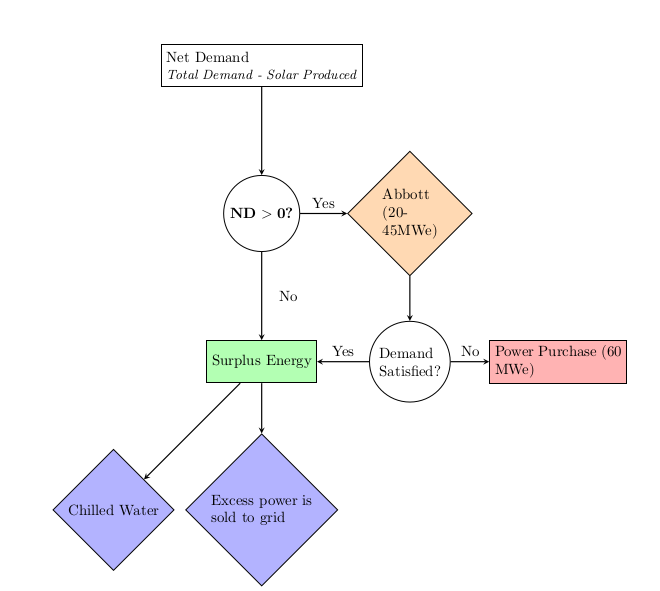
\includegraphics[width=\linewidth]{../figures/campus_grid_breakdown.png}
		\captionof{figure}{A flow chart describing the current campus energy grid.}
	\end{minipage}
	\begin{minipage}{0.48\linewidth}
		\centering
		\label{fig:future_grid}
		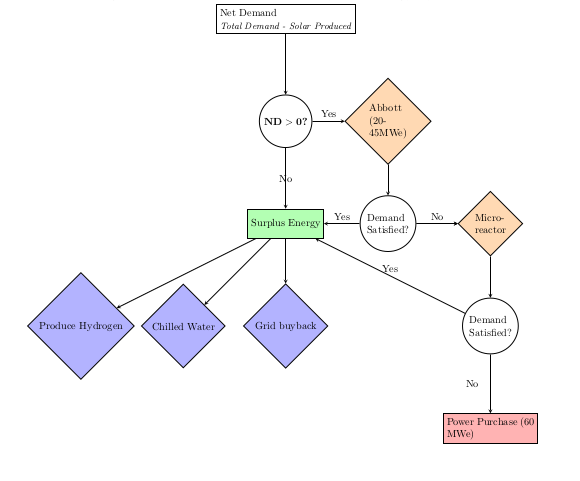
\includegraphics[width=\linewidth]{../figures/uiuc-es2.png}
		\captionof{figure}{A flow chart describing a potential grid with a micro-reactor.}
	\end{minipage}
\end{figure}

\vspace{1cm}
\textbf{Typical Years}\\

In order to generate a typical year of data, datasets for 2015-2018 with hourly resolution were passed
to the RAVEN framework which collected and evaluated each month of data to find the most ``typical'' 
month. These ``typical'' months were concatenated into a single year of data to get a ``typical year.''
This method aims to remove outliers due to extreme or unusual weather conditions \cite{alfonsi_raven_2016}\cite{baker_optimal_2018}. 

\vspace{0.7em}
\begin{figure}
	\centering
	\begin{minipage}{0.23\linewidth}
		\centering
		\label{fig:load}
		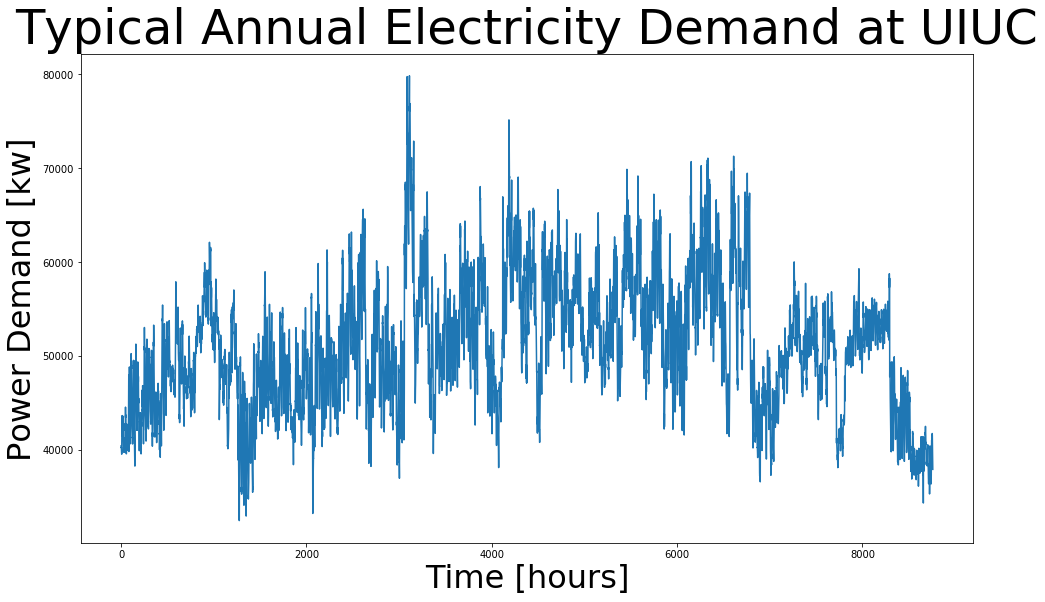
\includegraphics[width=\linewidth]{../figures/typical_demand.png}
		% \captionof{figure}{}
	\end{minipage}
	\begin{minipage}{0.23\linewidth}
		\centering
		\label{fig:steam}
		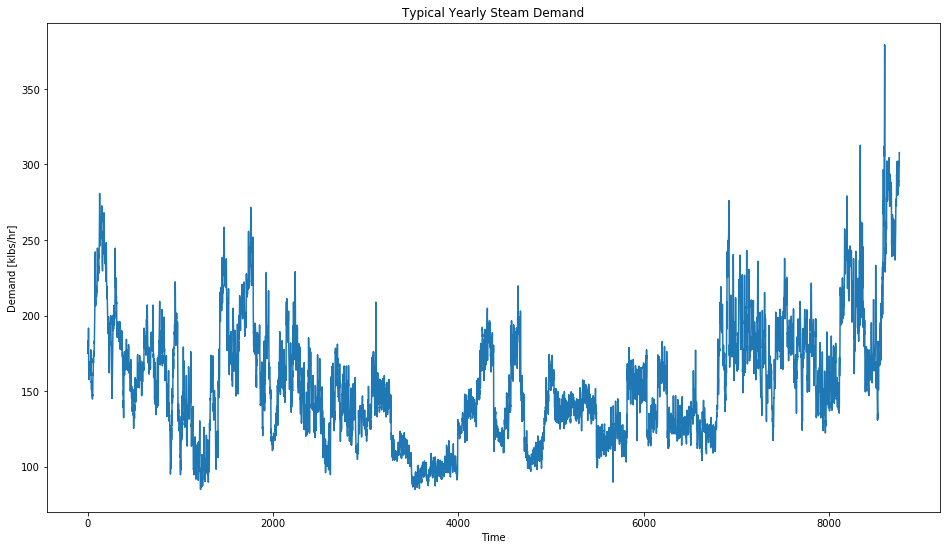
\includegraphics[width=\linewidth]{../figures/typical_steam.png}
		% \captionof{figure}{}
	\end{minipage}
	\begin{minipage}{0.23\linewidth}
		\centering
		\label{fig:solar}
		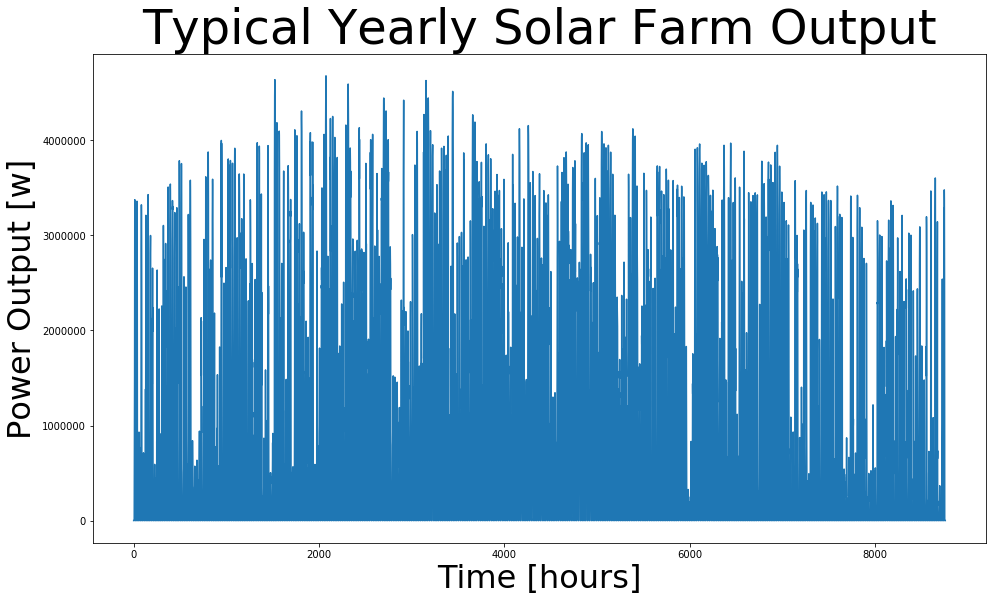
\includegraphics[width=\linewidth]{../figures/typical_solarpower.png}
		% \captionof{figure}{}
	\end{minipage}
	\begin{minipage}{0.23\linewidth}
		\centering
		\label{fig:temp}
		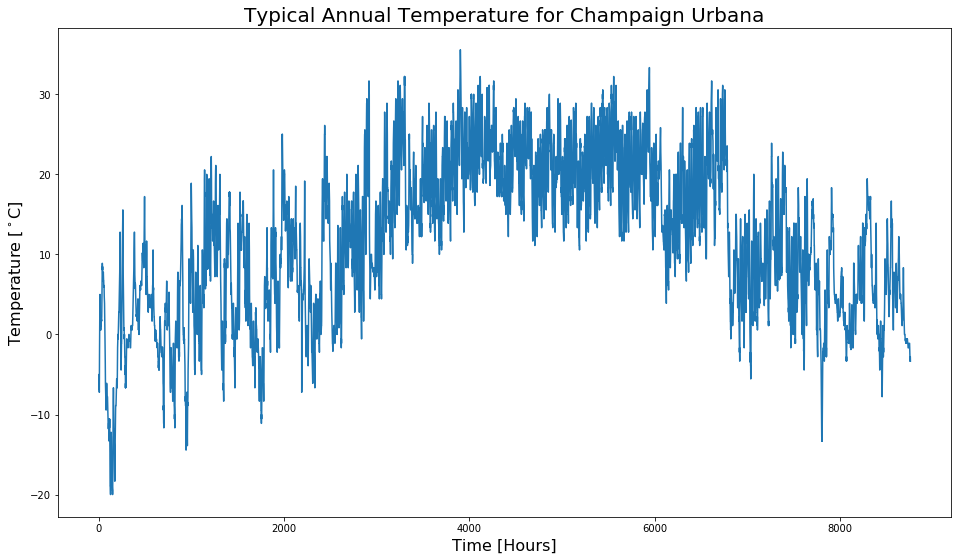
\includegraphics[width=\linewidth]{../figures/typical_weather.png}
		% \captionof{figure}{}
	\end{minipage}
	\caption{A typical year of data for quantity \textit{\textbf{X}}. Generated using the RAVEN framework.\cite{baker_optimal_2018}}
\end{figure}

\textbf{Modelling Solar Farm Output}\\

In order to fill gaps in the real output of the the power output was calcuated using solar irradiance data. The model tends to underpredict the power output but generally gets the correct shape, which lends credence to the irradiance data.
\begin{figure}[H]
	\centering
	\label{fig:model-comparison}
	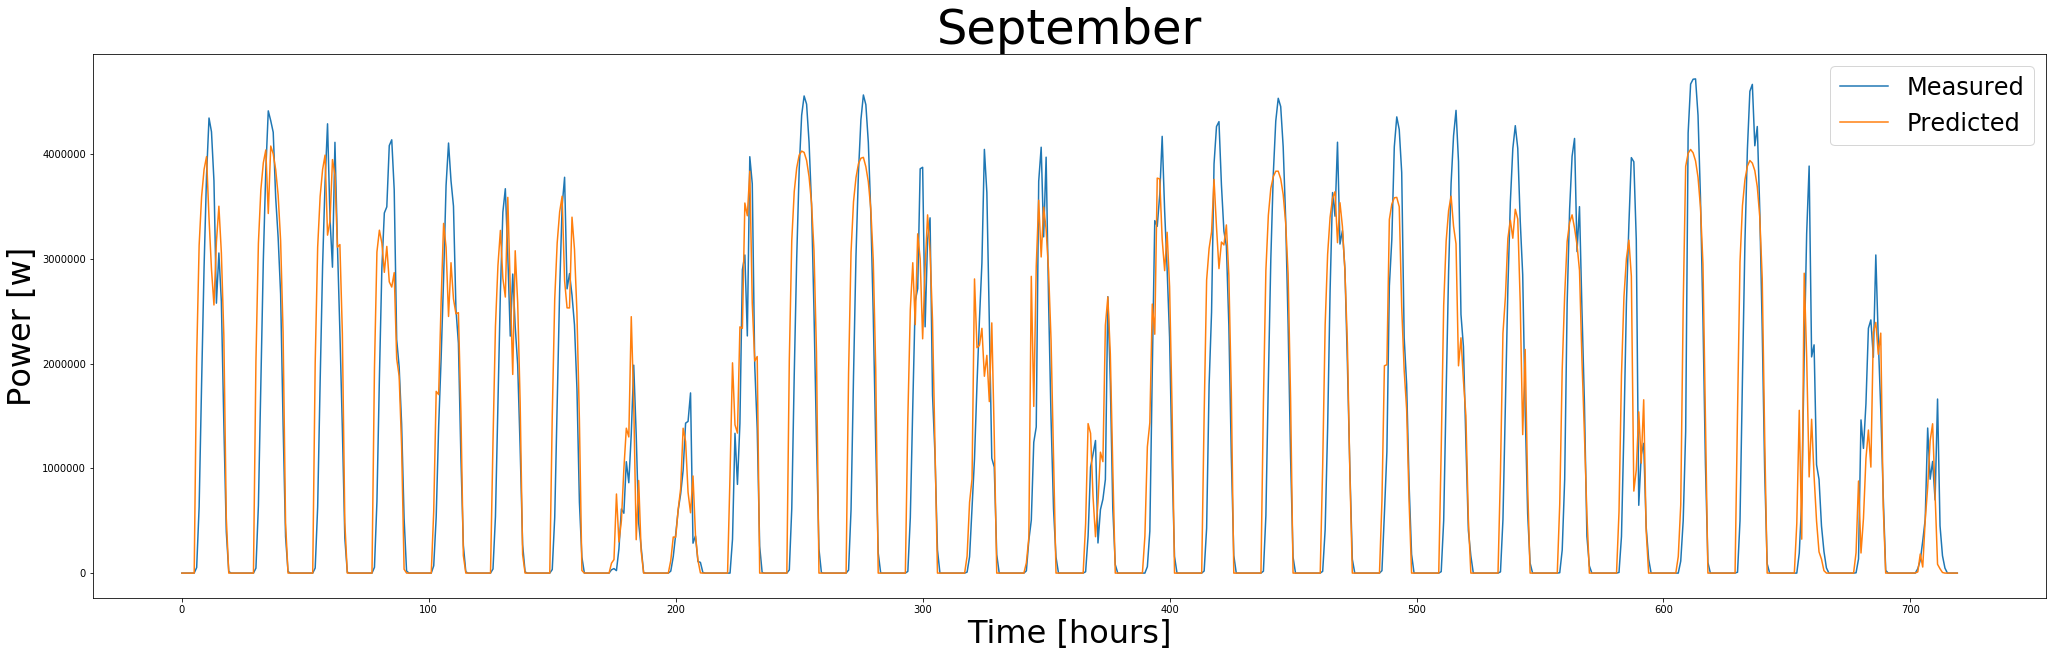
\includegraphics[width=\linewidth]{../figures/september_model_comparison.png}
	\caption{Comparing the predicted power output with the actual power output for September 2016}
\end{figure}

\end{block}

\end{column} % End of column 2
%----------------------------------------------------------------------------------------

\begin{column}{\sepwid}\end{column} % Empty spacer column

\begin{column}{\onecolwid} % The third column

\begin{block}{Methods}
\vspace{0.7em}
\textbf{Modelling Solar Farm Output}\\
The campus solar farm offers publicly available data about it's output \cite{alsoenergy_university_2019}, but there are several
long periods of missing data. In order to fill this missing data I collected data from Open Energy 
Information (OpenEI) \cite{noauthor_national_nodate} about the solar irradiance in Champaign-Urbana.
To get the power output from the solar irradiance the following equations were used \cite{garcia_nuclear_2015}: 

\begin{equation}
 \delta = 23.44\sin\left(\left(\frac{\pi}{180}\right)\left(\frac{360}{365}\right)(N+284)\right) \text{ } \left[degrees \right]	
\end{equation}
\small{\begin{itemize}
 	\item $\delta$ is the solar declination (``how high in the sky'').
 	\item $N$ is the day number (January 1st is 1, and so on).
 	\item The factor of $\frac{\pi}{180}$ is a conversion factor.
 \end{itemize} }


\begin{equation}
	G_T = DNI*\cos\left(\beta+\delta-lat\right) + DHI*\left(\frac{180-\beta}{180}\right) \text{ } \left[\frac{W}{m^2}\right]
\end{equation}
\small{
	\begin{itemize}
		\item $G_T$ is the total solar irradiance
		\item $DNI$ is the \textit{direct normal irradiance}.
		\item $DHI$ is the \textit{diffuse horizontal irradiance}.
		\item $\beta$ is the tilt angle of the solar panel.
	\end{itemize}
}

\begin{equation}
	P = G_T\eta_{ref}\tau_{pv}A\left[1-\gamma\left(T-25\right)\right] \text{ } \left[W\right]
\end{equation}

\small{
	\begin{itemize}
		\item $\eta$, $\tau$, $\gamma$ are solar panel properties (efficiency, transmittance, and temperature coefficient, respectively).
		\item $A$ is the area coverage of the solar panels.
	\end{itemize}
}


\end{block}


%----------------------------------------------------------------------------------------
%	ACKNOWLEDGEMENTS
%----------------------------------------------------------------------------------------

\setbeamercolor{block title}{fg=norange,bg=white} % Change the block title color

\begin{block}{Acknowledgements}
	
This work was made possible with data provided by UIUC Facilities and Services, 
in particular, Morgan White, Mike Marquissee, and Mike Larson. Additionally, 
this work is funded by the NRC Fellowship Program.  
	
\end{block}

%----------------------------------------------------------------------------------------
%	CONTACT INFORMATION
%----------------------------------------------------------------------------------------


\begin{block}{References}

	{\footnotesize\bibliographystyle{abbrv} 
	\bibliography{poster}}
\end{block}


%----------------------------------------------------------------------------------------



\end{column} % End of the third column

\end{columns} % End of all the columns in the poster

\end{frame} % End of the enclosing frame

\end{document}
\begin{column}{\sepwid}\end{column} % Empty spacer column
